\documentclass[a4paper,12pt]{article} % тип документа

% Поля страниц
\usepackage[left=2.5cm,right=2.5cm, top=2cm,bottom=2cm,bindingoffset=0cm]{geometry}

%Пакет дял таблиц   
\usepackage{multirow} % Слияние строк в таблице
\newcommand{\eds}{\ensuremath{ \mathscr{E}}}
\newcommand{\ga}{\ensuremath{\gamma}}
\usepackage{tikz} 
\usepackage{array,tabularx,tabulary,booktabs} % Дополнительная работа с таблицами
\usepackage{longtable}  % Длинные таблицы
\usepackage{multirow} % Слияние строк в таблице
%Отступ после заголовка    
\usepackage{indentfirst}


% Рисунки
\usepackage{subcaption,floatrow,graphicx,calc}
\usepackage{wrapfig}

% Создаёем новый разделитель
\DeclareFloatSeparators{mysep}{\hspace{1cm}}

% Ссылки?
\usepackage{hyperref}
%\usepackage[rgb]{xcolor}
%  Русский язык
\usepackage[T2A]{fontenc}			% кодировка
\usepackage[utf8]{inputenc}			% кодировка исходного текста
\usepackage[english,russian]{babel}	% локализация и переносы


% Математика
\usepackage{amsmath,amsfonts,amssymb,amsthm,mathtools, mathrsfs, wasysym}

\author{Гаврилин Илья\\
	Добровольская Ксения\\
	Б01-110}
\title{\textbf{Лабораторная работа 5.1.3\\ 
		Изучение рассеяния медленных электронов на атомах (эффект Рамзауэра)}}

\begin{document}
	\maketitle
	\paragraph*{Цель работы: } Получить ВАХ эффекта на экране ЭО, измерить расстояния между характерными точками в вольтах; снять ВАХ в статическом режиме; по результатам измерений рассчитать размер электронной оболочки атома, оценить глубину потенциальной ямы и потенциал ионизации газа, заполняющего лампу.
	\section*{Теория}
	\subsection*{Эффект Рамзауэра}
	\textit{Эффективное сечение реакции} --- это величина, характеризующая вероятность перехода системы двух сталкивающихся частиц в результате их рассеяния (упругого или неупругого) в определенное конечное состояние. Сечение $\sigma$ это отношение числа таких переходов $N$ в единицу времени к плотности потока $nv$ рассеиваемых частиц, падающих на мишень, т.е. к числу частиц, падающих в единицу времени на единичную площадку, перпендикулярно к их скорости.
	
	\begin{equation}
		\sigma = \frac{N}{nv}
	\end{equation}
	
	Эффект Рамзауэра нельзя объяснить с позиции классической теории. С квантовой же точки зрения картина рассеяния выглядит следующим образом: внутри атома потенциальная энергия падающего электрона отлична от нуля, скорость электрона меняется, становясь равной $v'$ в соответствии с законом сохранения энергии 
	
	\[E = \frac{mv^2}{2} = \frac{mv'^2}{2}+U\]
	
	а значит, изменяется и длина его волны де-Бройля. Таким образом, по отношению к электронной волне атом ведет себя как преломляющая среда с относительным показателем преломления
	\begin{equation}
		n = \frac{\lambda}{\lambda'} = \sqrt{1 - \frac{U}{E}}
	\end{equation}
	
	Решение задачи о рассеянии электрона на сферическом потенциале достаточно громоздко. Поэтому рассматривают более простое одномерное приближение: электрон рассеивается на потенциальной яме конечной глубины. После решения соответствующего уравнения Шрёдингера получается выражение для коэффициента прохождения:
	
	\begin{equation}
		D = \frac{16 k_1^2 k_2^2}{16k_1^2 k_2^2 + 4\left(k_1^2-k_2^2\right)^2\sin^2\left(k_2 l\right)}
	\end{equation}
	где $k_1^2 = \frac{2mE}{\hbar^2}, k_2^2 = \frac{2m(E + U_0)}{\hbar^2}$.
	
	Как легко видно, это периодическое выражение с максимумами при 
	
	\begin{equation}
		k_2 l = \pi n = \sqrt{\frac{2m(E + U_0)}{\hbar^2}}l
	\end{equation}
	
	Это же условие можно получить, рассматривая интерференцию двух волн --- прошедшей через атом и отраженной от границ атомного потенциала. Тогда получаются следующие выражения для эффективного размера атома $l$:
	\begin{equation}
		2l = \frac{h}{\sqrt{2m(E_1 + U_0)}}
	\end{equation}
	
	\begin{equation}
		2l = \frac{3}{2}\frac{h}{\sqrt{2m(E_2 + U_0)}}
	\end{equation}
	
	Где $E_1, E_2$ --- энергии, соответствующие максимуму и минимуму прохождения электронов соответственно. Исключая $U_0$ можно найти 
	
	\begin{equation}
		l = \frac{h\sqrt{5}}{\sqrt{32m(E_2 - E_1)}}
	\end{equation}
	
	А исключая $l$ можно найти эффективную глубину потенциальной ямы атома:
	
	\begin{equation}
		U_0 = \frac{4}{5}E_2 - \frac{9}{5}E_1
	\end{equation}
	
	Так же можно вывести теоретически формулу, связывающую зависимость вероятности рассеяния электрона от его энергии:
	\begin{equation}
		w(V) = -\frac{1}{C} \ln \frac{I_a(V)}{I_0}
	\end{equation}
	
	С помощью неё, имея ВАХ тиратрона, можно построить график $w(V)$.
	
	\section*{Схема установки}
	Лампа-тиратрон ТГ301/1.3Б, заполненная инертным газом, расположена непосредственно на корпусе блока источников питания (БИП). Напряжение к электродам лампы подаются от источников питания, находящиеся в корпусе прибора. Регулировка напряжения и выбор режима работы установки производится при помощи ручек управления, выведенных на лицевую панель БИП.
	
	\begin{figure}[H]
		\begin{center}
			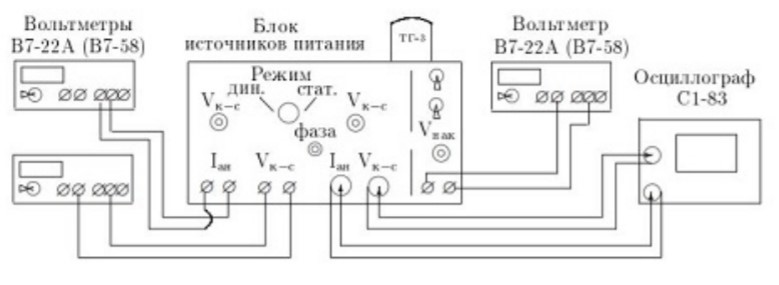
\includegraphics[width = 0.6\textwidth]{3.jpg}
			\caption{Блок-схема экспериментальной установки}
		\end{center}
	\end{figure}
	\section*{Ход работы}
	\subsection*{Динамический режим}
	Снимем с помощью осциллографа ВАХ при двух различных напряжениях, а затем измерим $U_{\max}$, $U_{\min}$ в зависимости от $U_{\text{накала}}$. Все данные занесем в таблицу.
	\begin{table}[H]
		\centering
		\begin{tabular}{|c|c|c|}
			\hline
			$U$, В & $U_max$, В & $U_min$, В \\ \hline
			2.60 & 2.0       & 6.0       \\ \hline
			2.83 & 2.0       & 7.0       \\ \hline
		\end{tabular}
		\caption{Показания в динамическом режиме}
	\end{table}
	Используя полученные данные и формулы (7) - (8) рассчитаем $l$ и $U_0$.
	\begin{table}[H]
		\centering
		\begin{tabular}{|c|c|c|}
			\hline
			$U$, В     & 2.6  & 2.83 \\ \hline
			$l$, \r{A}  & 3.43 & 3.07 \\ \hline
			$U_0$, эВ & 1.2  & 2    \\ \hline
		\end{tabular}
		\caption{Результаты вычисления $l$, $U_0$}
	\end{table}
	Сравним полученные результаты с табличными значениями.
	\begin{table}[H]
		\centering
		\begin{tabular}{|c|c|c|}
			\hline
			& $l$, \r{A}      & $U_0$, эВ   \\ \hline
			эксперимент & $3.25 \pm 0.21$ & $1.6 \pm 0.1$ \\ \hline
			теория      & 3.8       & 2.5        \\ \hline
		\end{tabular}
	\caption{Сравнение результатов, полученных в динамическом режиме}
	\end{table}
	Перейдем к статическому режиму.
	\subsection*{Статический режим}
	Проведем измерение при двух значениях напряжения накала ($U_\text{нак}$), результаты занесем в таблицу. По полученным данным построим графики, по ним определим максимальное и минимальное напряжение.
	\begin{table}[H]
		\centering
		\begin{tabular}{|cc|cc|}
			\hline
			\multicolumn{2}{|c|}{$U_\text{нак}   = 2.60$ В} & \multicolumn{2}{c|}{$U_\text{нак}   = 2.83$ В} \\ \hline
			\multicolumn{1}{|c|}{$I$, отн. ед.}       & $U$, В      & \multicolumn{1}{c|}{$I$, отн. ед.}      & $U$, В     \\ \hline
			\multicolumn{1}{|c|}{0.1}     & 0.0    & \multicolumn{1}{c|}{0.1}    & 0.0   \\ \hline
			\multicolumn{1}{|c|}{0.3}     & 0.5    & \multicolumn{1}{c|}{0.5}    & 0.5   \\ \hline
			\multicolumn{1}{|c|}{42.0}    & 1.0    & \multicolumn{1}{c|}{54.6}   & 1.0   \\ \hline
			\multicolumn{1}{|c|}{166.5}   & 1.6    & \multicolumn{1}{c|}{175.0}  & 1.5   \\ \hline
			\multicolumn{1}{|c|}{174.1}   & 1.7    & \multicolumn{1}{c|}{184.5}  & 1.8   \\ \hline
			\multicolumn{1}{|c|}{157.1}   & 2.0    & \multicolumn{1}{c|}{182.2}  & 1.9   \\ \hline
			\multicolumn{1}{|c|}{164.8}   & 1.9    & \multicolumn{1}{c|}{183.9}  & 1.6   \\ \hline
			\multicolumn{1}{|c|}{170.6}   & 1.9    & \multicolumn{1}{c|}{187.1}  & 1.7   \\ \hline
			\multicolumn{1}{|c|}{175.2}   & 1.8    & \multicolumn{1}{c|}{186.8}  & 1.7   \\ \hline
			\multicolumn{1}{|c|}{99.9}    & 2.6    & \multicolumn{1}{c|}{170.5}  & 2.1   \\ \hline
			\multicolumn{1}{|c|}{70.7}    & 3.0    & \multicolumn{1}{c|}{137.7}  & 2.6   \\ \hline
			\multicolumn{1}{|c|}{51.2}    & 3.6    & \multicolumn{1}{c|}{115.2}  & 3.1   \\ \hline
			\multicolumn{1}{|c|}{40.9}    & 4.1    & \multicolumn{1}{c|}{98.3}   & 3.6   \\ \hline
			\multicolumn{1}{|c|}{35.1}    & 4.6    & \multicolumn{1}{c|}{85.1}   & 4.2   \\ \hline
			\multicolumn{1}{|c|}{31.7}    & 5.1    & \multicolumn{1}{c|}{79.8}   & 4.5   \\ \hline
			\multicolumn{1}{|c|}{29.3}    & 5.6    & \multicolumn{1}{c|}{73.4}   & 5.1   \\ \hline
			\multicolumn{1}{|c|}{24.6}    & 6.2    & \multicolumn{1}{c|}{69.8}   & 5.6   \\ \hline
			\multicolumn{1}{|c|}{27.3}    & 6.7    & \multicolumn{1}{c|}{67.7}   & 6.1   \\ \hline
			\multicolumn{1}{|c|}{27.4}    & 7.1    & \multicolumn{1}{c|}{67.8}   & 6.5   \\ \hline
			\multicolumn{1}{|c|}{27.6}    & 7.5    & \multicolumn{1}{c|}{67.7}   & 7.1   \\ \hline
			\multicolumn{1}{|c|}{29.2}    & 8.1    & \multicolumn{1}{c|}{67.8}   & 6.7   \\ \hline
			\multicolumn{1}{|c|}{31.0}    & 8.6    & \multicolumn{1}{c|}{70.4}   & 7.5   \\ \hline
			\multicolumn{1}{|c|}{33.2}    & 9.1    & \multicolumn{1}{c|}{74.7}   & 8.1   \\ \hline
			\multicolumn{1}{|c|}{36.8}    & 9.6    & \multicolumn{1}{c|}{79.9}   & 8.6   \\ \hline
			\multicolumn{1}{|c|}{45.7}    & 10.1   & \multicolumn{1}{c|}{87.7}   & 9.1   \\ \hline
			\multicolumn{1}{|c|}{47.0}    & 10.6   & \multicolumn{1}{c|}{95.9}   & 9.6   \\ \hline
			\multicolumn{1}{|c|}{55.5}    & 11.2   & \multicolumn{1}{c|}{119.2}  & 10.1  \\ \hline
			\multicolumn{1}{|c|}{61.0}    & 11.6   & \multicolumn{1}{c|}{127.0}  & 11.2  \\ \hline
			\multicolumn{1}{|c|}{}        &        & \multicolumn{1}{c|}{148.6}  & 11.2  \\ \hline
		\end{tabular}
		\caption{Результаты замеров в статическом режиме}
	\end{table}
	На построенных графиках определим координаты максимума и минимума, используя их рассчитаем $l$, $U_0$.
	\begin{table}[H]
		\centering
		\begin{tabular}{|c|c|c|}
			\hline
			$U$, В     & $l$, \r{A} & $U_0$, эВ  \\ \hline
			2.60   & $3.1 \pm 0.2$  & $2.1 \pm 0.3$     \\ \hline
			2.83  & $3.1 \pm 0.2$ & $2.1 \pm 0.3$     \\ \hline
			среднее   & $3.1\pm 0.2$  & $2.1 \pm 0.3$     \\ \hline
			табличное & 3.8  & 2.5     \\ \hline
		\end{tabular}
	\caption{Результаты в статическом режиме}
	\end{table}
	\begin{figure}[H]
		\centering
		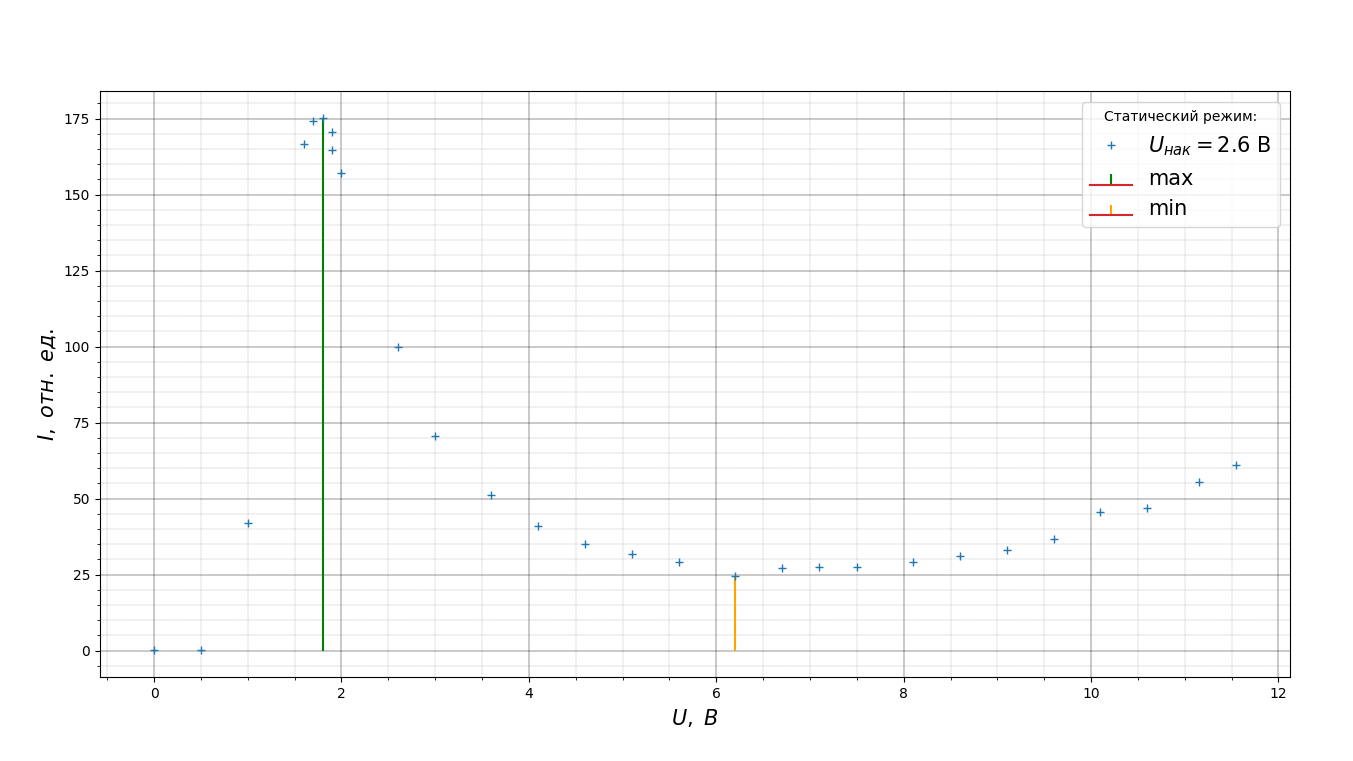
\includegraphics[width=0.85\linewidth]{graph_1}
		\caption{Результаты при $U_\text{нак} = 2.60$ В}
		\label{fig:graph1}
	\end{figure}
	\begin{figure}[H]
		\centering
		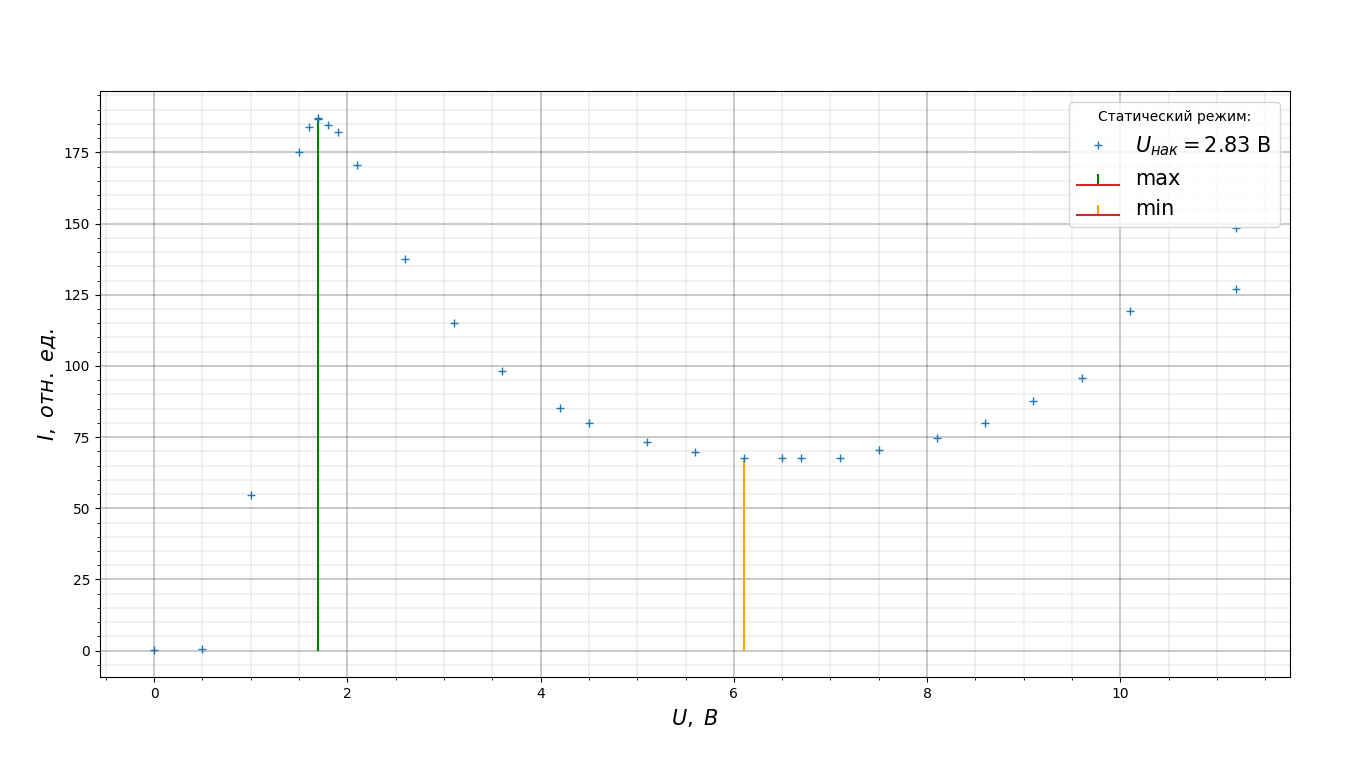
\includegraphics[width=0.85\linewidth]{graph_2}
		\caption{Результаты при $U_\text{нак} = 2.83$ В}
		\label{fig:graph2}
	\end{figure}
	Используя формулу (9) можем построить зависимость вероятности рассеяния от напряжения, приведем качественный график.
	\begin{figure}[H]
		\centering
		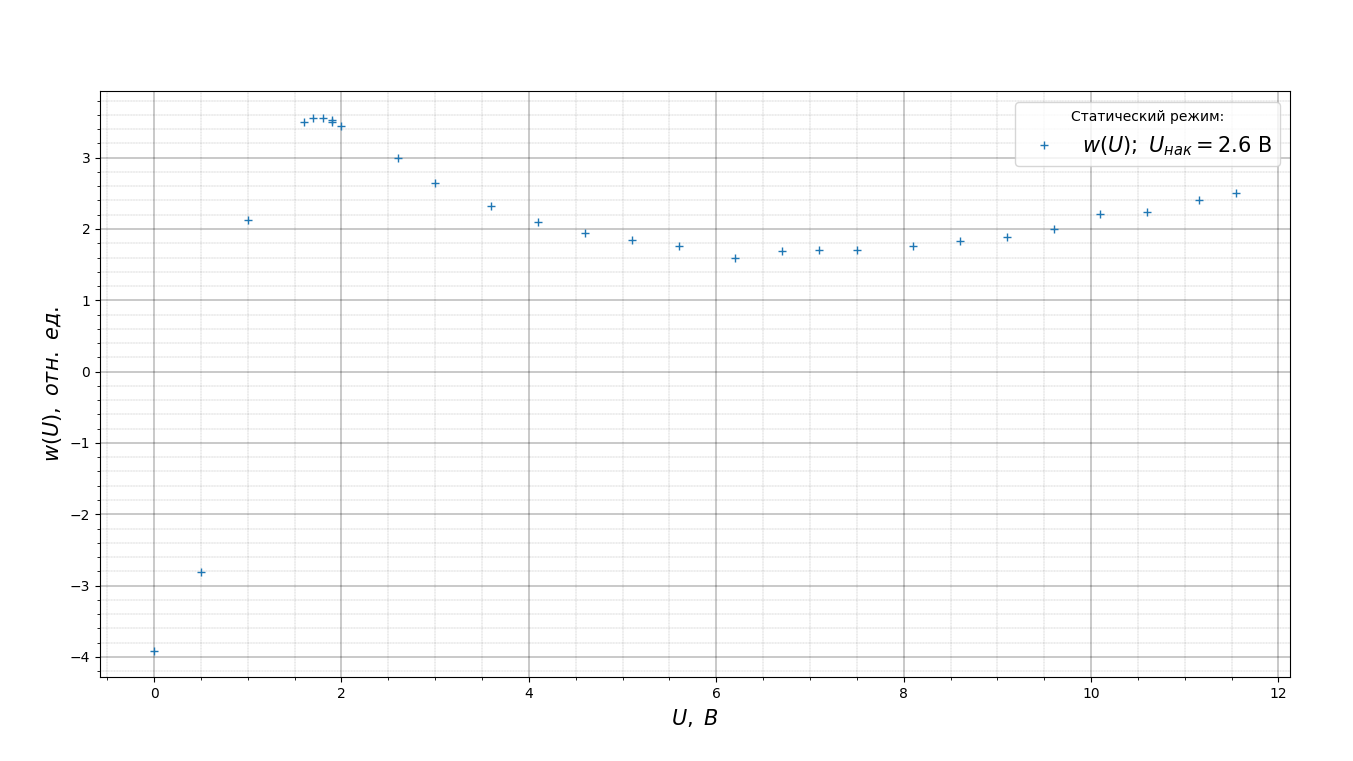
\includegraphics[width=0.85\linewidth]{graph_3}
		\caption{Качественная зависимость $w(U)$}
		\label{fig:graph3}
	\end{figure}
	\section*{Выводы}
	В данной лабораторной работе была получена ВАХ эффекта Рамзауэра на экране осциллографа в динамическом режиме. \\
	Для динамического режима были рассчитаны
	размер электронной оболочки атома $l = (3.25 \pm 0.21)$ \r{A}, глубина потенциальной ямы
	$U_0 = 1.6 \pm 0.1$ эВ.\\
	Была снята ВАХ в статическом режиме. По результатам измерений рассчитан
	размер электронной оболочки атома $l = (3.1 \pm 0.2)$ \r{A}, а также глубина потенциальной
	ямы $U_0 = 2.1 \pm 0.3$ эВ.\\
	Табличные значения для данных величин составляют: $l = 3.8$ \r{A}, $U_0 = 2.5$ эВ. Экспериментальные данные немного отличны от табличных.\\
	Также в ходе работы были оценены значения энергий, при которых должны
	появляться максимумы в коэффициенте прохождения электоронов для $n =2$, $n =3$,
	что соответственно составляют следующие величины (из формулы (4)): $E_2=13.5$ эВ, $E_3=32.9$ эВ.\\
	Более того, была получена качественная зависимость вероятности рассеяния электрона от напряжения на тиратроне.
\end{document}